\section{Bestiaire}

\subsection{Pilier de bar Horoxien} \label{sec:horoxian-barfly}
\begin{figure}[h!]
    \centering
    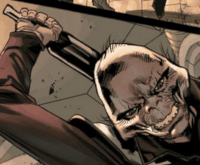
\includegraphics[height=200pt]{_img/bestiary/horoxian-barfly.png}
\end{figure}
\paragraph{Background}
Pas très malin, le pilier de bar horoxian se cache dans les cantina d’Horox III. Passe le plus clair de son temps à picoler et à refaire le monde avant de retourner à sa pauvre vie dénuée d’intérêt. C’est pourquoi dès que l’occasion se présente d’engager une bagarre, peu importe la raison, le pilier de bar Horoxien n’hésite pas \dots Bien bourré, le pilier de bar Horoxien ne sent pas la douleur, il n’est pas gêné par ses blessures.

\paragraph{Traits}

\begin{itemtable}[ c c c c c ]
    \textbf{Agi} & \textbf{Int} & \textbf{\^Ame} & \textbf{For} & \textbf{Vig} \\
    d4           & d4           & d4             & d8           & d8
\end{itemtable}
\begin{itemtable}[ l X ]
    \textbf{Allure}      & 6 \\
    \textbf{Compétences} & Combat d6
\end{itemtable}

\paragraph{Défense}
\begin{itemtable}[ c c ]
    \textbf{Parade}     & \textbf{Résistance} \\
    5 (-1 Alcool)       & 6
\end{itemtable}

\paragraph{Arme possible}
\begin{itemtable}[ X c c ]
    ~                & \textbf{Dégats} \\
    Bouteille cassée & 2d8
\end{itemtable}


\newpage

\subsection{Garde de la citadelle} \label{sec:citadel-guard}
\begin{figure}[h!]
    \centering
    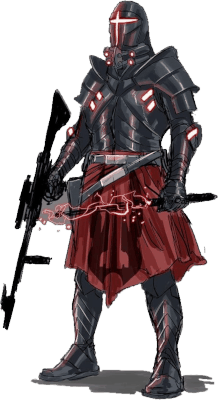
\includegraphics[height=200pt]{_img/bestiary/citadel-guard.png}
\end{figure}
\paragraph{Background}
Gardes au service de la reine. Ne parlent pas, ne réfléchissent pas et obéissent sans poser de questions aux ordres de \nameref{sec:bombinax}. Formés au combat depuis leur plus tendre enfance, les gardes de la citadelle sont équipés d’une armure lourde qui ne leur permet pas une grande liberté de mouvement mais leur confère une protection intégrale.

\paragraph{Traits}

\begin{itemtable}[ c c c c c ]
    \textbf{Agi} & \textbf{Int} & \textbf{\^Ame} & \textbf{For} & \textbf{Vig} \\
    d4           & d4           & d4             & d8           & d8
\end{itemtable}
\begin{itemtable}[ l X ]
    \textbf{Allure}      & 6 \\
    \textbf{Compétences} & Combat d10, Tir d8
\end{itemtable}

\paragraph{Défense}
\begin{itemtable}[ c c ]
    \textbf{Parade}     & \textbf{Résistance} \\
    7                   & 6 (+4)
\end{itemtable}

\paragraph{Arme possible}
\begin{itemtable}[ X c c ]
    ~                   & \textbf{Dégats} \\
    Fusil laser         & 2d8 + 2 \\
    Matraque neurale    & 1d6 + 1
\end{itemtable}

\newpage
\subsection{Symbiote Abersyn} \label{sec:symbiote-abersyn}
\begin{figure}[h]
    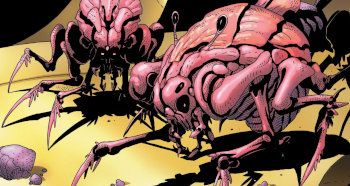
\includegraphics[width=\linewidth]{_img/bestiary/symbiote-abersyn.jpg}
\end{figure}

\subsubsection{Background}
Ces bestioles, grosses comme le poing sont bêtes et méchantes. Pas très dangereuses en soi mais si elles vous attrapent, elles s’immiscent en vous, viennent s’accrocher à votre cortex cérébral et prennent votre place aux commandes de votre corps. La bonne nouvelle est que vous ne mourrez pas, vous restez pleinement conscient de tout ce qu’il se passe sans pouvoir y faire quoi que ce soit.

\subsubsection{Combat}
Ces saletés n’ont pas de traits, elles ne sont pas jouées en combat comme des ennemis normaux. Elles n’apparaissent qu’en groupe, n’importe quelle attaque qui touche les explose. Par contre elles viennent perturber les combats.

Le MJ tire une carte pour tout le groupe de Symbiote. Quand c’est à leur tour de jouer, le MJ lance un dé (d2, d4, d6, \dots selon le nombre de créature présentent). Le résultat indique combien de joueurs sont attaqués par l’une de ces créatures. Elles attaquent avec \textbf{d6} à opposer à la \textbf{Par}ade de l’adversaire. Si l’adversaire ne pare pas, il n’y a pas de dégâts mais celui-ci, à son tour, doit réussir un jet de \textbf{Bag}arre pour se débarrasser du symbiote avant de pouvoir attaquer une cible différente. Il y passera son action tant qu’il ne réussit pas.